 \documentclass[12pt,a4paper,twoside]{article}
\input{spp.dat}
\usepackage{graphicx}
\usepackage{subcaption}
\usepackage{amssymb, amsmath}
\usepackage{siunitx}
\usepackage{physics}

\begin{document}

\title{\TitleFont Input-Output response of a system
}

\author[ ]{Kenneth Domingo\authorsep}
\author[ ]{Rhei Joven Juan\authorsep}
\author[ ]{Rene Principe Jr.\lastauthorsep}
\affil[ ]{National Institute of Physics, University of the Philippines, Diliman, Quezon City}

\begin{abstract}
\noindent


\keywords{}

\end{abstract}

\maketitle
\thispagestyle{titlestyle}

\section{Introduction}
\label{sec:Intro}

One way of characterizing the overall performance of an instrument is by looking at its static and dynamic characteristics \cite{IDC}. Static characteristics mainly tackles about how the output changes with respect to the input. This can graphically be represented as the Input-Output (I/O) response curve of the system and its behaviour is a direct hint as to how stable, accurate, precise, linear, selective, etc. the operating system is \cite{Sensors}.

On the other hand, the dynamic characteristics describe the transient properties of a system where the input or the "measurand" is changing with respect to time \cite{Sensors}. This is common for a system with energy-storing components such inductors and capacitors  that has behaviours described by a differential equation (either zero, first, seconds, or higher orders) \cite{Sensors}. For example, First-Order circuits such as a loaded Resistor-Inductor (RL) circuit and a loaded Resistor-Capacitor (RC) circuit will have a natural discharging response given by the Kirchoffs Voltage Law (KVL) equations respectively.

\begin{equation}\label{eq:kvl-rl}
    L\dv{I_L}{t} + RI_L = 0
\end{equation}

\begin{equation}\label{eq:kvl-rc}
    RC\dv{V_C}{t} + V_C = 0
\end{equation}

where $L$ is the inductance, $I_L$ is the current on the inductor, $R$ is the resistance value of the respective resistor, $C$ is the capacitance, while $V_C$ is the voltage across the capacitor \cite{1stODE}.  

In this study, linearity of components such as resistors, capacitors, inductors, and LEDs' shall be determined by generating their I/O curves.

\medskip

\section{Methodology}
\label{sec:Metho}
Using the Wheatstone bridge circuit, the input and output signals were measured using the probes of an oscilloscope at the input voltage and at $R_T$. A triangle wave was generated having a maximum amplitude of 2.5\si{\volt} at the lowest possible frequency. This was used as input to the circuit. The probe in Channel 1 was used to observe the input signal while the probe in Channel 2 was used to observe the output signals, at the specific points stated before. The oscilloscope was then set to X-Y mode and the input-output curve was plotted using the obtained data from the oscilloscope. This was then compared to the same set-up but having the amplitude of the input signal to 1.5 times the original amplitude. The methodology was done while varying $R_T$ using various passive electrical devices, such as a resistor, capacitor, and inductor, with circuit diagrams shown in Figures \ref{fig:wheat-res}-\ref{fig:wheat-ind}.

\section{Results and Discussion}
\label{sec:RnD}
\medskip
Figures \ref{fig:res-lo} and \ref{fig:res-hi} show the I/O curves for a regular Wheatstone bridge with a 1000 Hz square input voltage $V_{in}$ of 2.5 and 3.75 V, respectively. In the phase diagram, the data points are concentrated in the upper right and lower left corners and sparse in between due to a square wave's rapid change in voltage. If interpolation were to be performed, Figure \ref{fig:res-lo} might appear elliptical, while Figure \ref{fig:res-hi} might appear more linear. Observation of the individual input and output curves on the left-hand side of the plot shows that the output mimics the input (implying linear response), and that they appear to be in-phase. However, the shape of the phase plot (unequal voltage rise and fall) on the right-hand side indicates that either they are roughly $\pi$ radians out of phase, or the Wheatstone bridge was not balanced and exhibits hysteresis. Increasing the input voltage does not affect the overall shape of the phase plot, so the resistor acts as a linear component.

Figures \ref{fig:cap-lo} and \ref{fig:cap-hi} show the I/O curves for a Wheatstone bridge, but with $R_T$ replaced with an integrator, i.e. same circuit as Figure \ref{fig:wheat-res} but with a capacitor connected in parallel with $R_T$ to the ground. Here, the elliptical shape of the phase plot is more defined, as a 100 Hz triangle wave was used for the input. This is mimicked by the output, which is now a sine wave with the same frequency (implying linear response), but with a slight phase difference which is reflected in the phase plot. The phase plot appearance is maintained when the input voltage is increased, so the capacitor acts as a linear component.

Figures \ref{fig:ind-lo} and \ref{fig:ind-hi} show the I/O curves for a Wheatstone bridge with $R_T$ replaced with an inductor. The input was maintained as a triangle wave, but the frequency was increased to 100 kHz, slightly beyond the resonant frequency of the RC circuit. This allowed the output waveform to still mimic that of the input, but now appears as a distorted sinusoid, where each rise and fall stage appears like a convex-right curve. The phase plot shows that the input and output are out of phase, and with the current conditions, the inductor behaves nonlinearly.

The major sources of error in this experiment stemmed from a faulty oscilloscope which kept corrupting connected portable storage devices, and the inductor, which initially produced noisy readings. Capacitive coupling from the breadboard may have also perturbed the readings.

\section{Conclusions}
\label{sec:Conc}
\medskip
\clearpage

\bibliographystyle{spp.bst}
\begin{thebibliography}{1}
\label{sec:Ref}

\bibitem[(IDC Techonologies(n.d.))]{IDC}
IDC Technologies (n.d.). Performance of Instruments: Static Characteristicss. Retrieved 3 March 2019, from \url{https://www.idc-online.com/technical_references/pdfs/instrumentation/Performance\%20of\%20Instruments_Static\%20Characteristics.pdf}


\bibitem[(K. Kalantar-zadeh)]{Sensors}
K. Kalantar-Zadeh (2013). Sensor Characteristics. \textit{Sensors; An Introductory Course. Springer, US}.  
doi: 10.1007/978-1-4614-5052-8

\bibitem[(F. Najmabadi(2001))]{1stODE}
F. Najmabadi (2001). Solution of First-Order Linear Differential Equation. \textit{Linear cicuit Theory}
Retrieved 3 March 2019, from \url{http://aries.ucsd.edu/najmabadi/CLASS/MAE140/NOTES/dynamic-2.pdf}

\end{thebibliography}

\clearpage

\section*{Appendix}

\begin{figure}[!h]
    \centering
    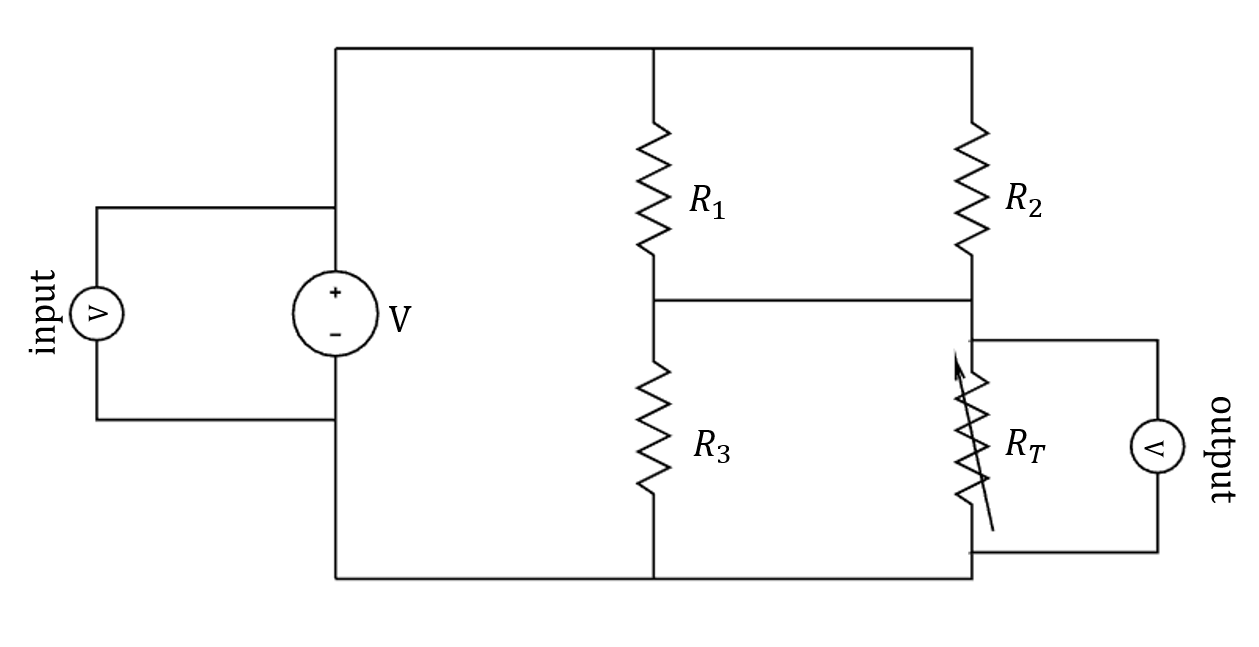
\includegraphics[width = 0.7\linewidth]{wheatstone-resistor.png}
    \caption{Schematic of a Wheatstone bridge circuit.}
    \label{fig:wheat-res}
\end{figure}

\begin{figure}[!h]
    \centering
    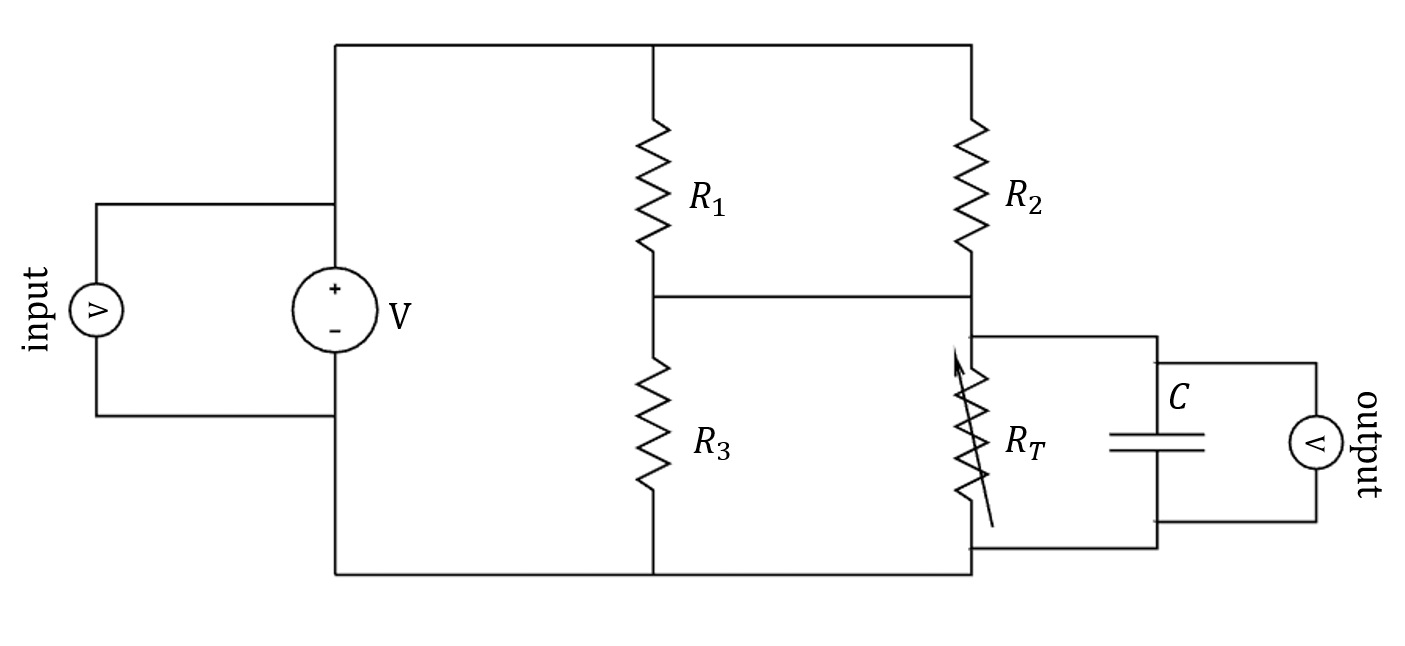
\includegraphics[width = 0.7\linewidth]{wheatstone-capacitor.png}
    \caption{Schematic of a Wheatstone bridge circuit.}
    \label{fig:wheat-cap}
\end{figure}

\begin{figure}[!h]
    \centering
    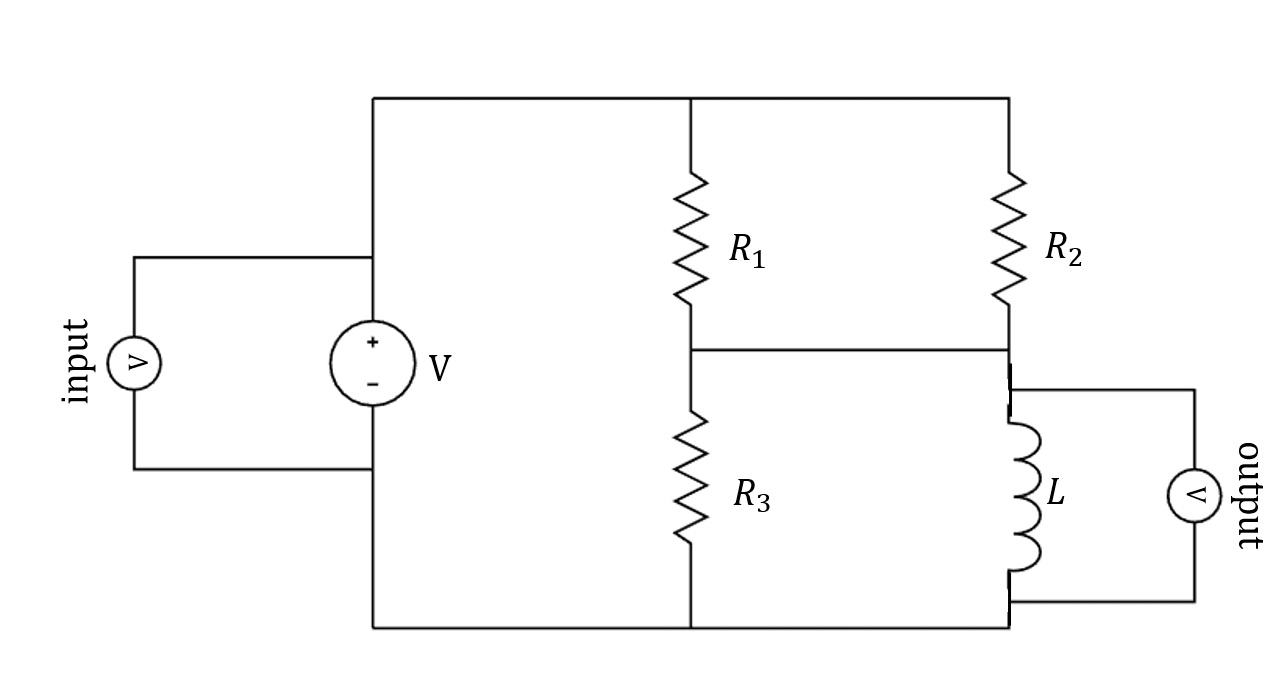
\includegraphics[width = 0.7\linewidth]{wheatstone-inductor.png}
    \caption{Schematic of a Wheatstone bridge circuit.}
    \label{fig:wheat-ind}
\end{figure}

\begin{figure}[!h]
    \centering
    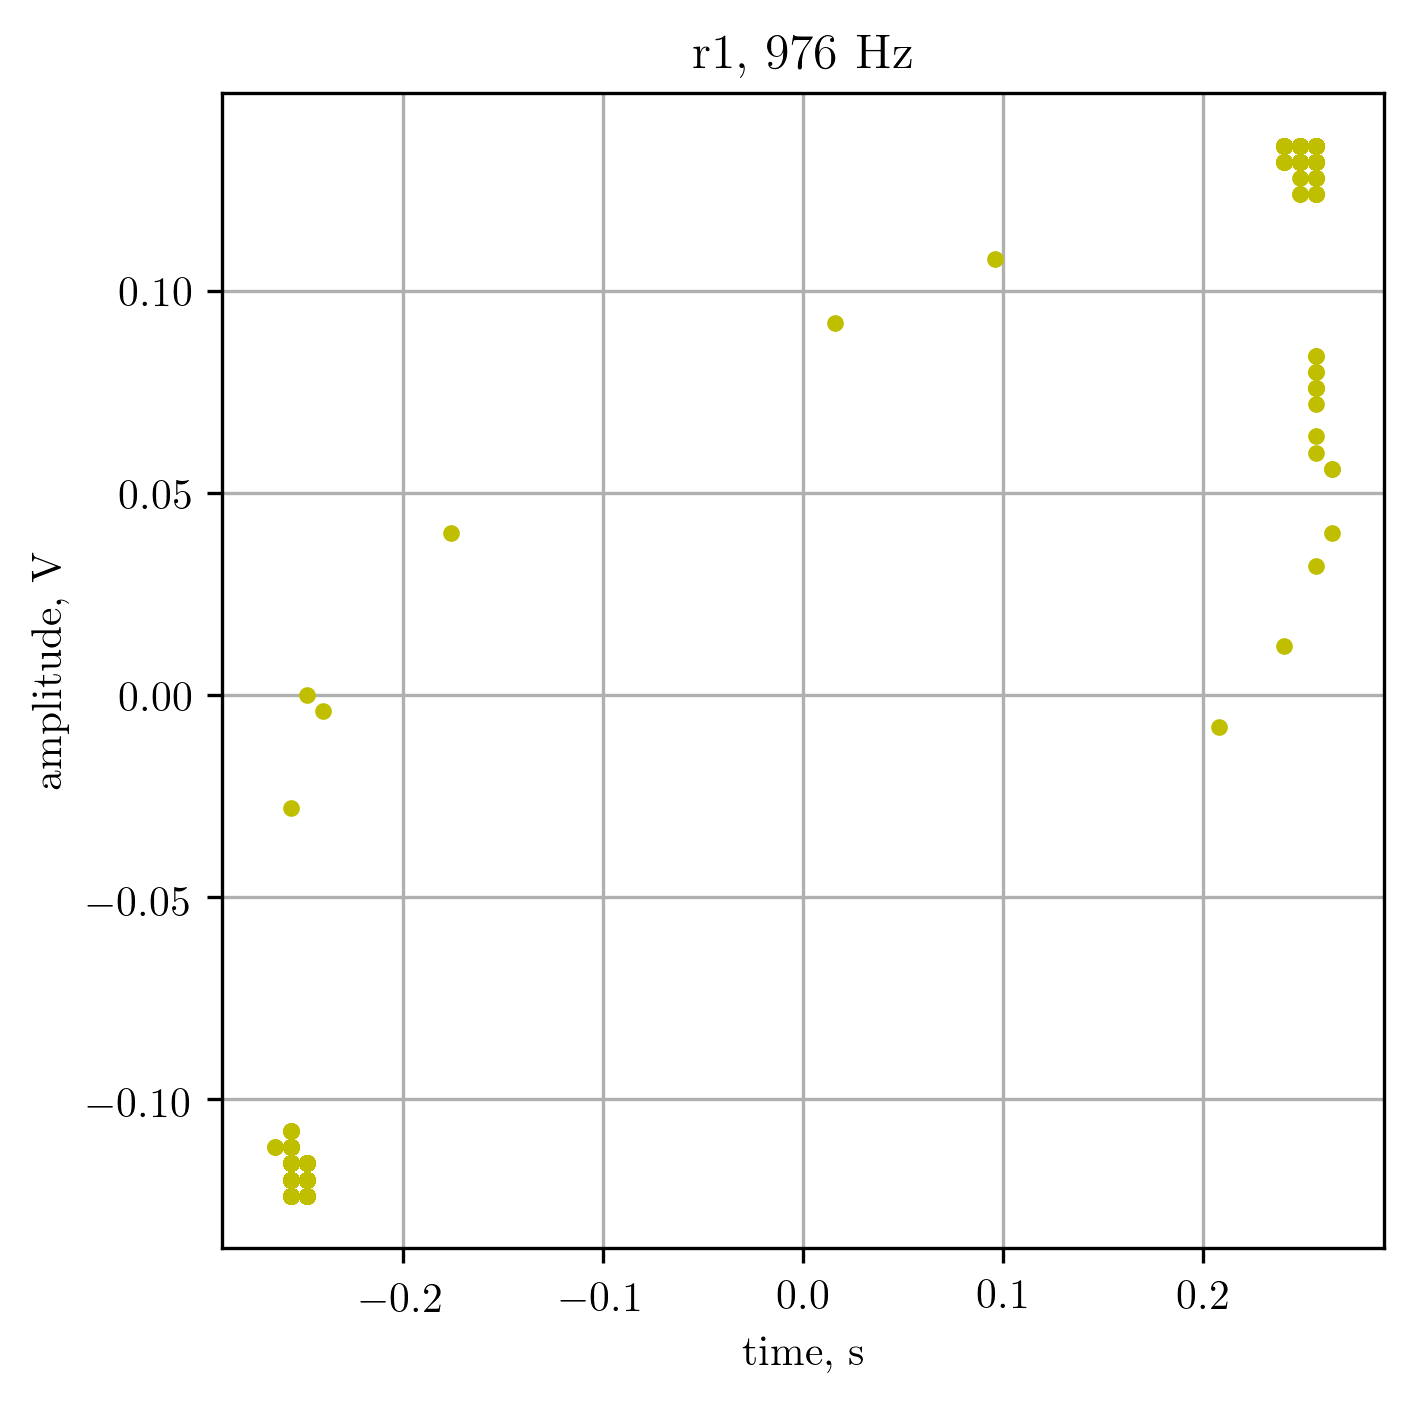
\includegraphics[width = \textwidth]{r1.png}
    \caption{Input-output curves of a regular Wheatstone bridge, $V_{in} = 2.5$ V.}
    \label{fig:res-lo}
\end{figure}

\begin{figure}[!h]
    \centering
    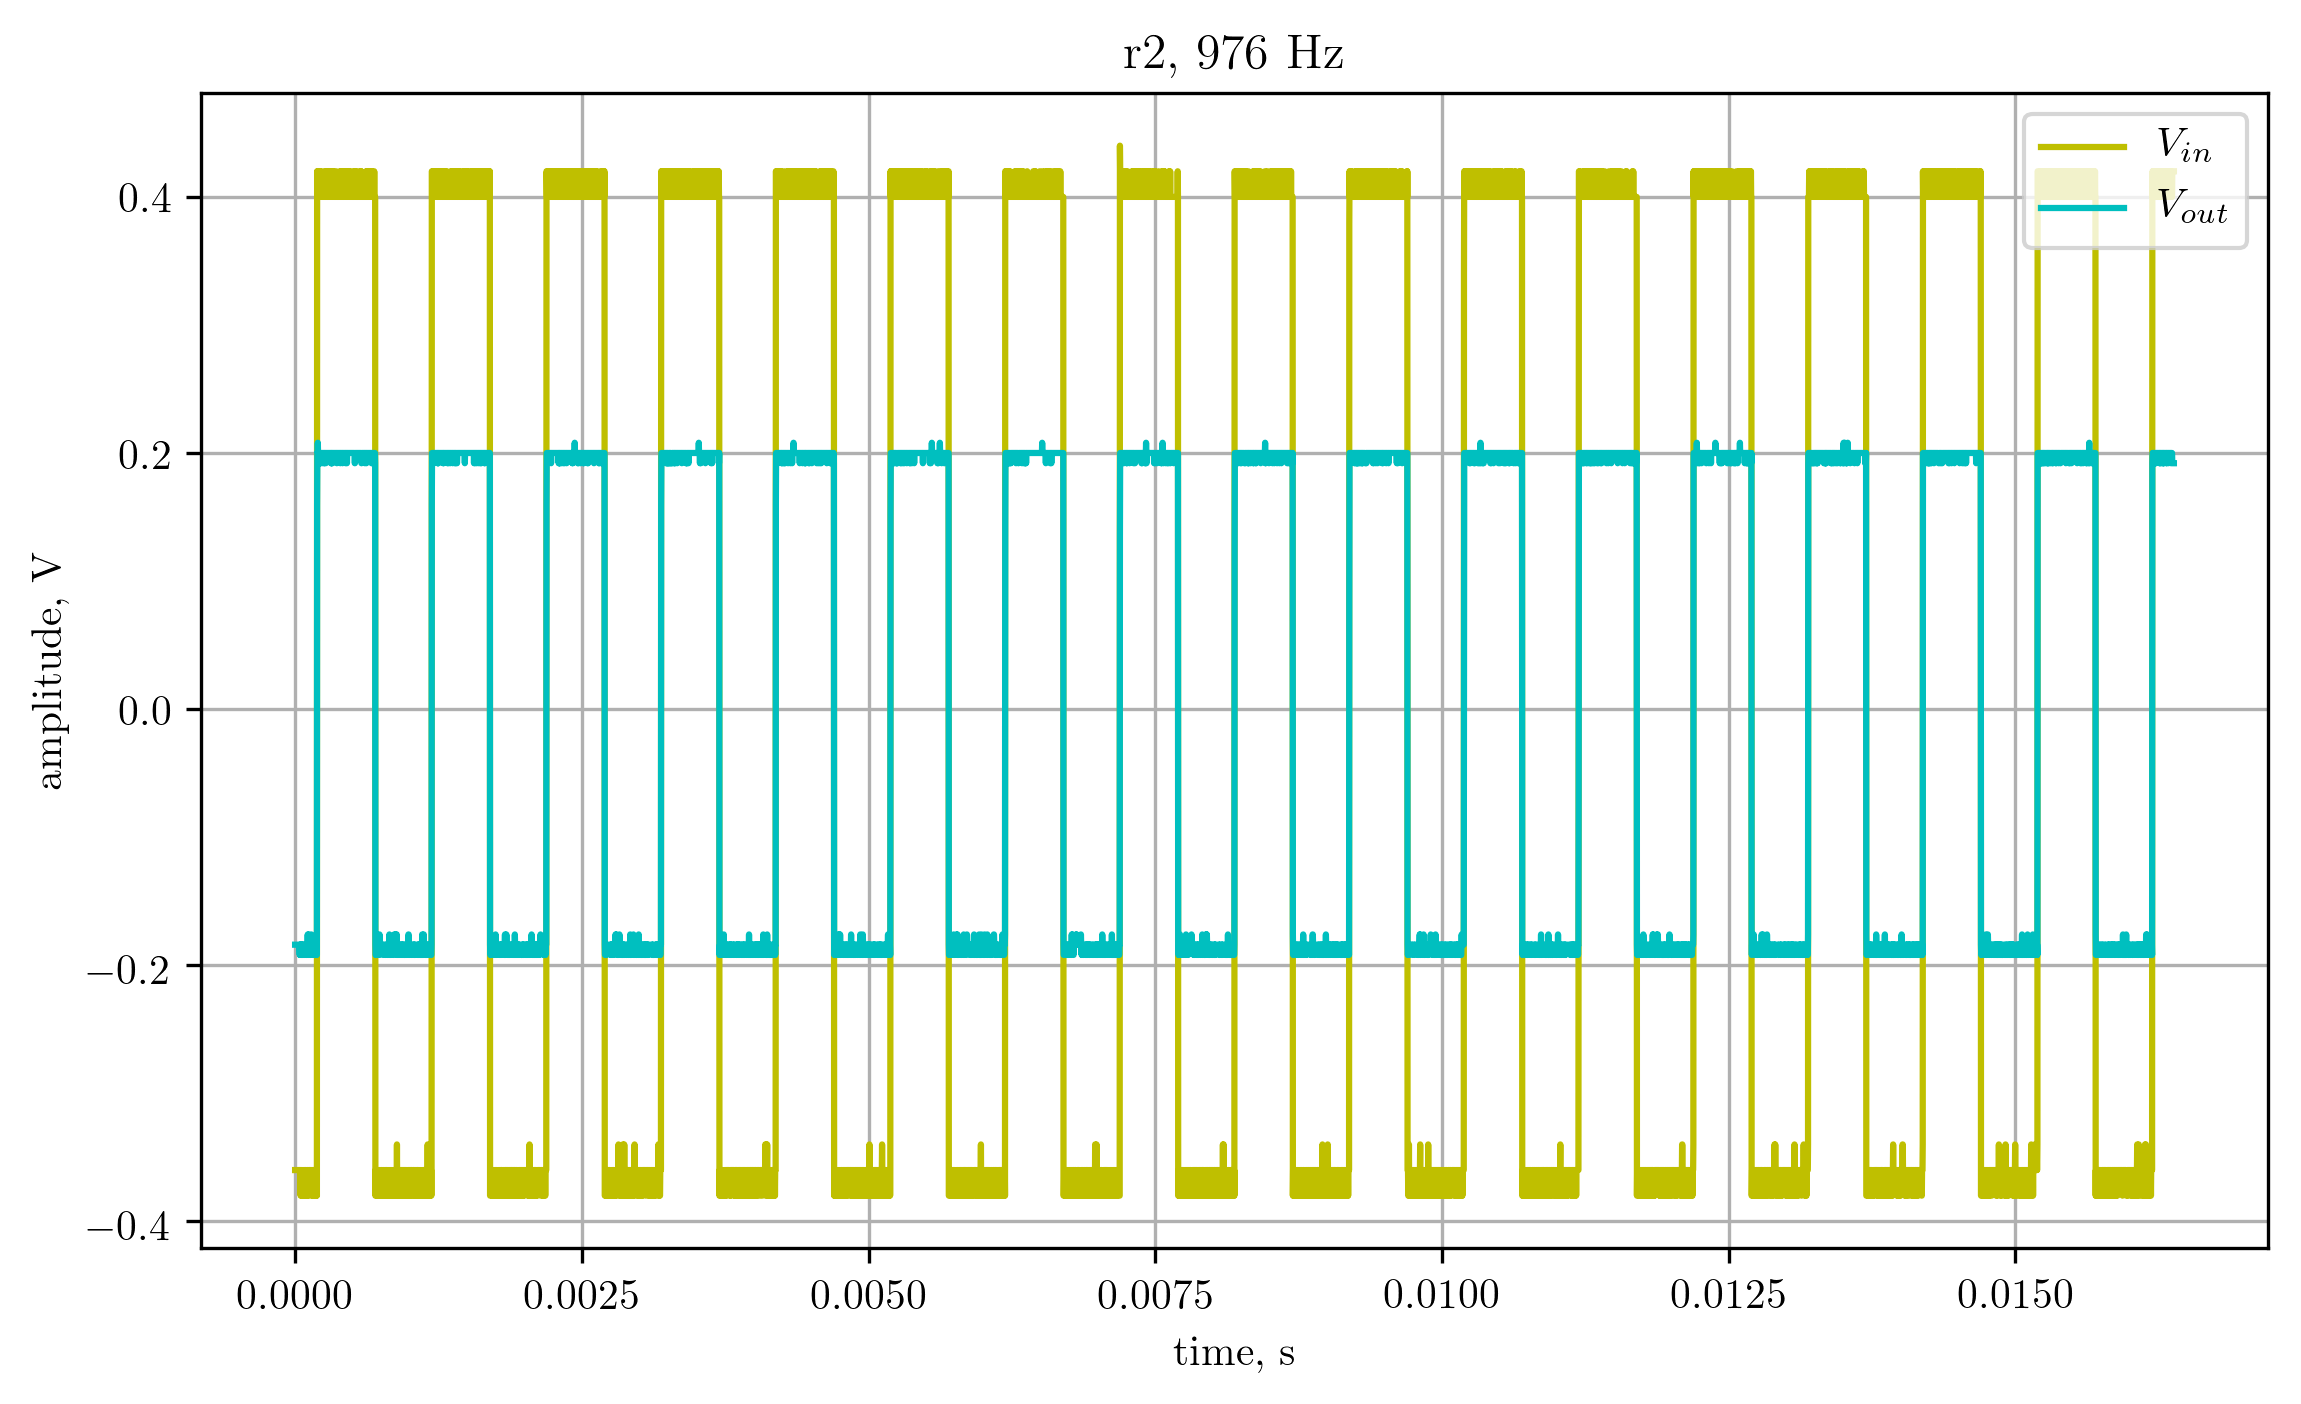
\includegraphics[width = \textwidth]{r2.png}
    \caption{Input-output curves of a regular Wheatstone bridge, $V_{in} = 3.75$ V.}
    \label{fig:res-hi}
\end{figure}

\begin{figure}[!h]
    \centering
    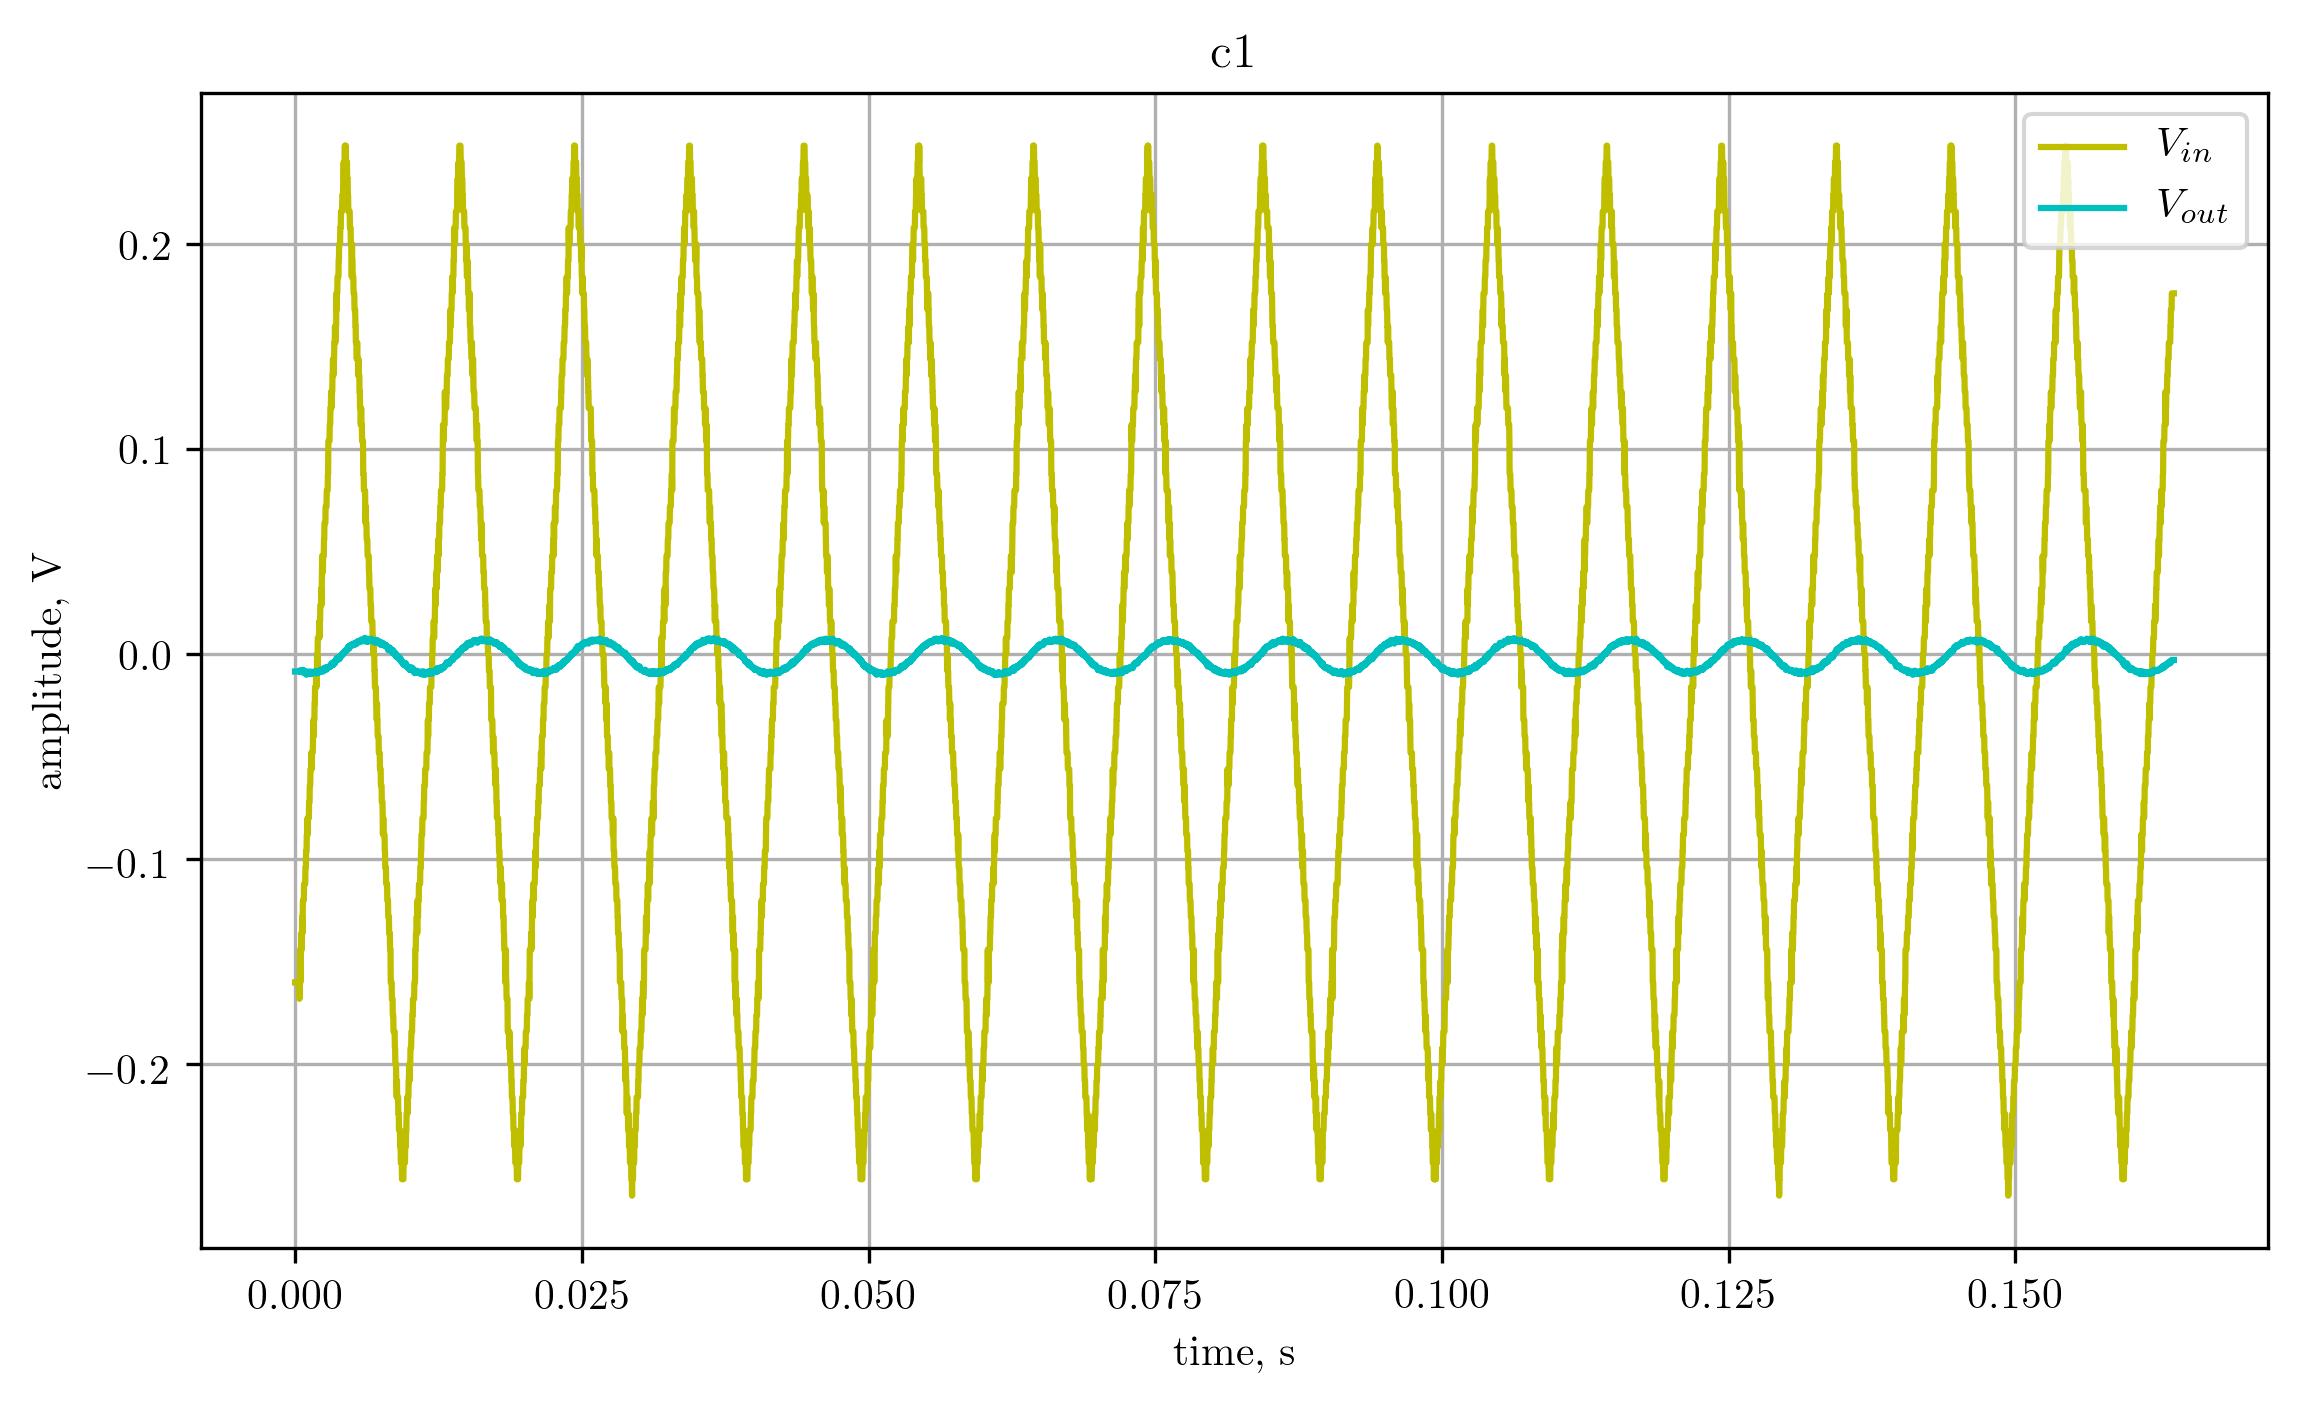
\includegraphics[width = \textwidth]{c1.png}
    \caption{Input-output curves of a Wheatstone bridge, $R_T$ replaced with an integrator filter, $V_{in} = 2.5$ V.}
    \label{fig:cap-lo}
\end{figure}

\begin{figure}[!h]
    \centering
    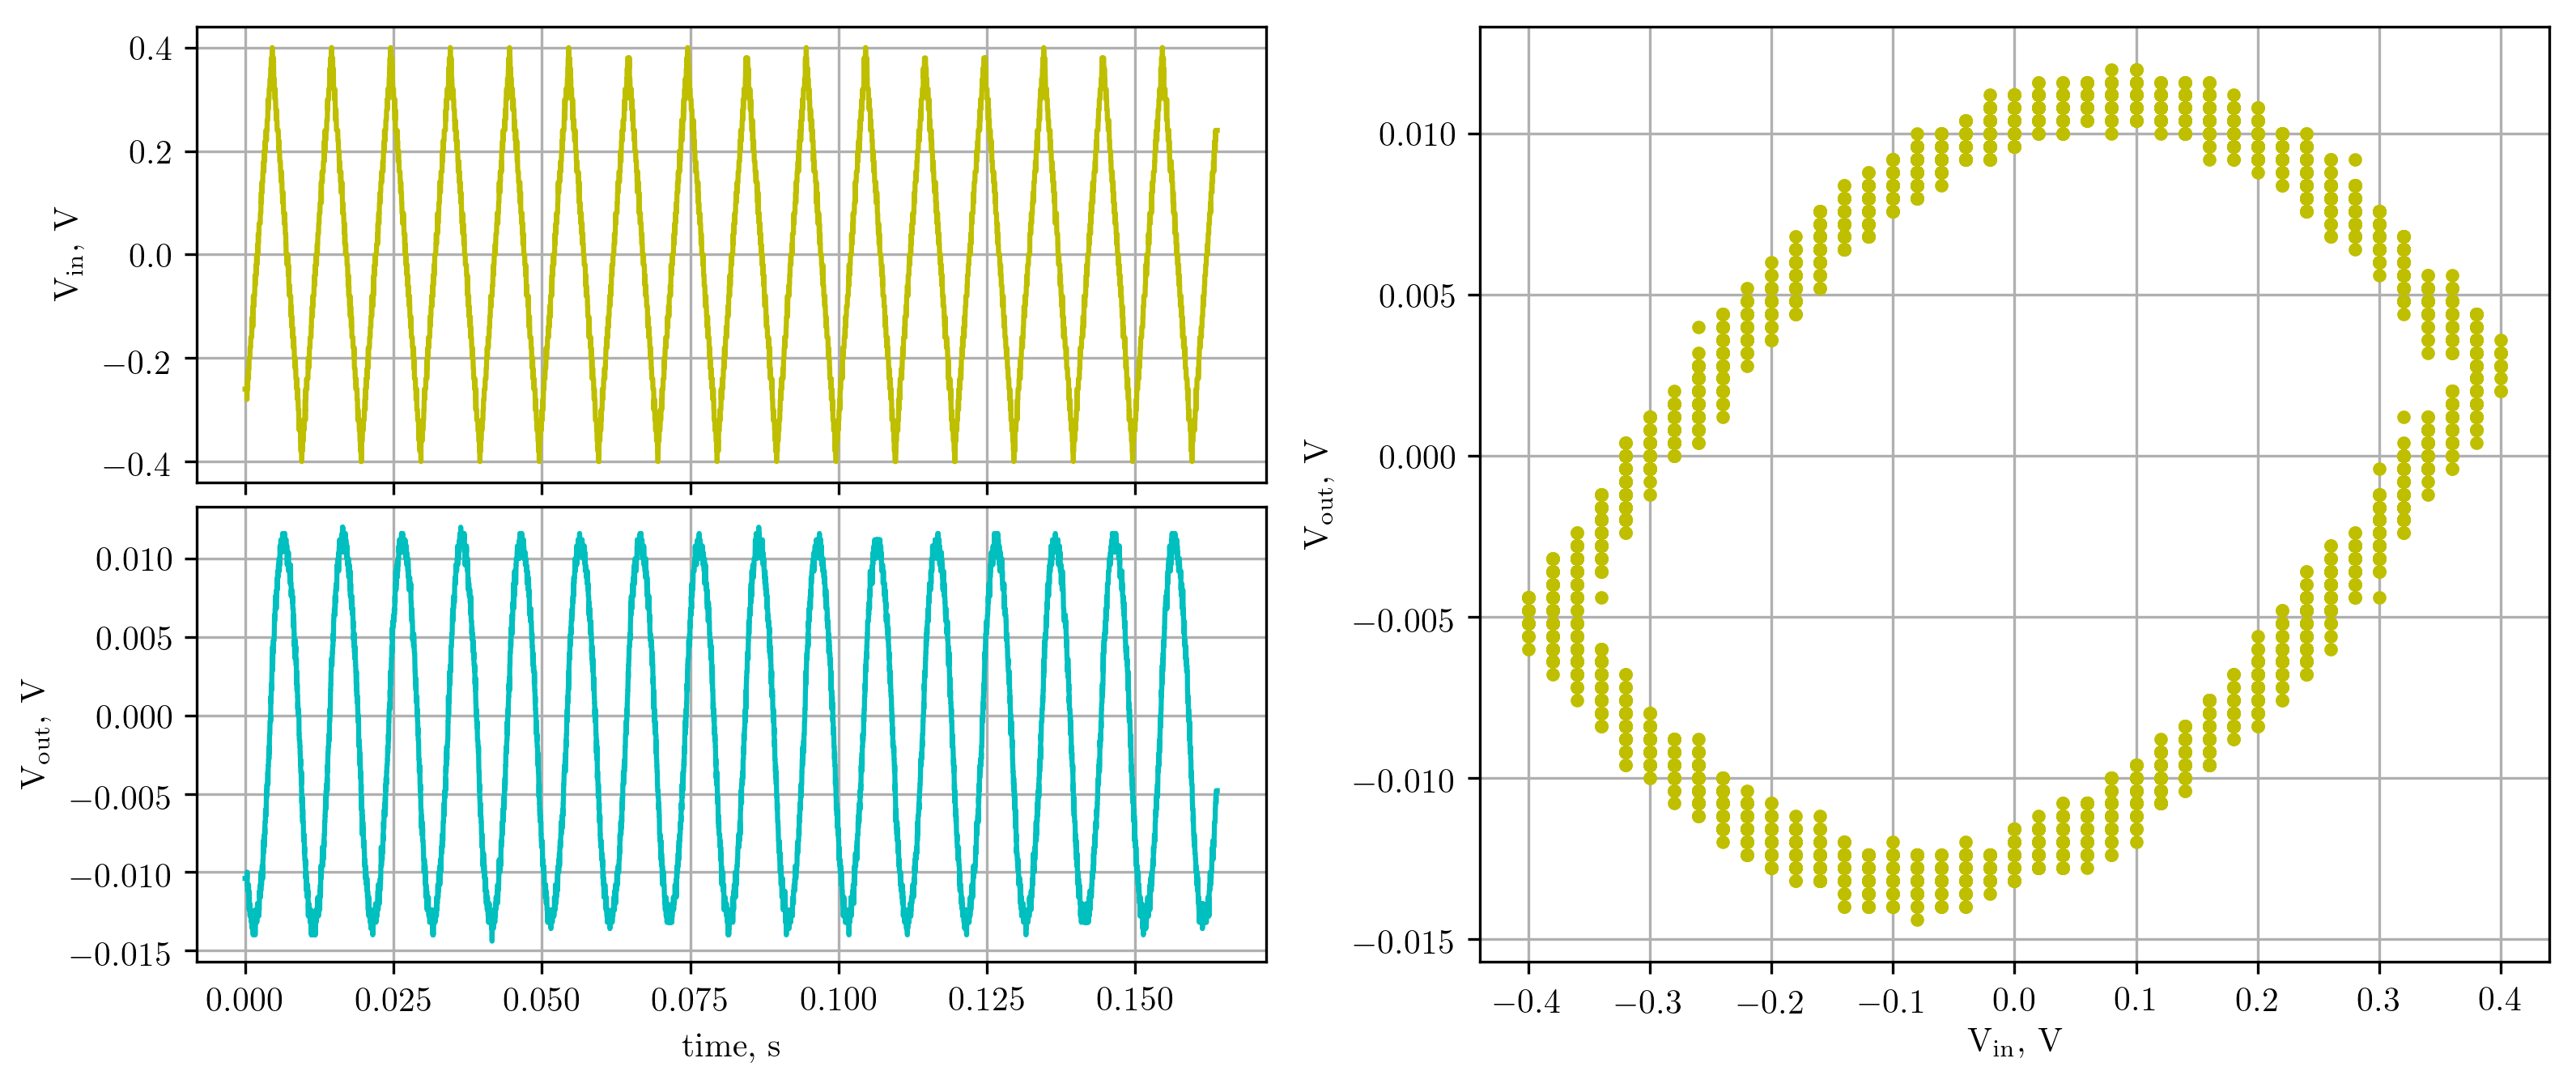
\includegraphics[width = \textwidth]{c2.png}
    \caption{Input-output curves of a Wheatstone bridge, $R_T$ replaced with an integrator filter, $V_{in} = 3.75$ V.}
    \label{fig:cap-hi}
\end{figure}

\begin{figure}[!h]
    \centering
    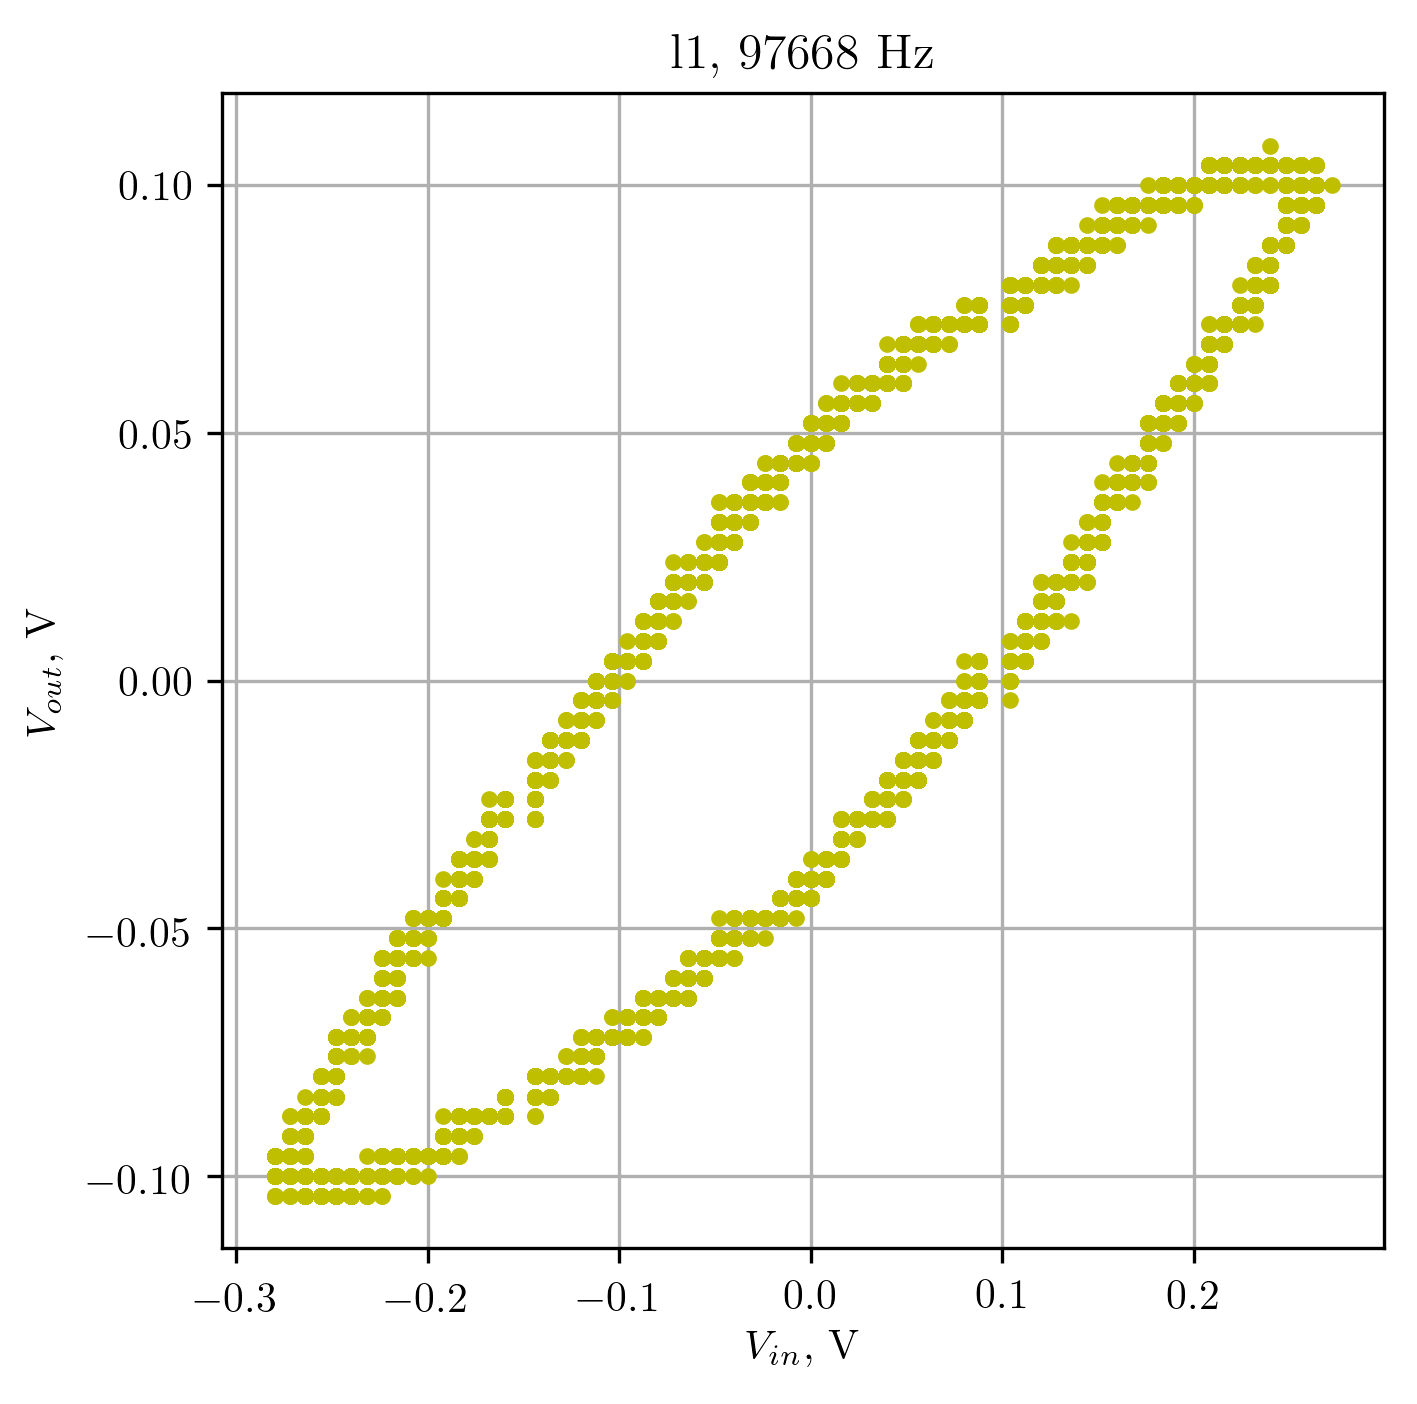
\includegraphics[width = \textwidth]{l1.png}
    \caption{Input-output curves of a Wheatstone bridge, $R_T$ replaced with an inductor, $V_{in} = 2.5$ V.}
    \label{fig:ind-lo}
\end{figure}

\begin{figure}[!h]
    \centering
    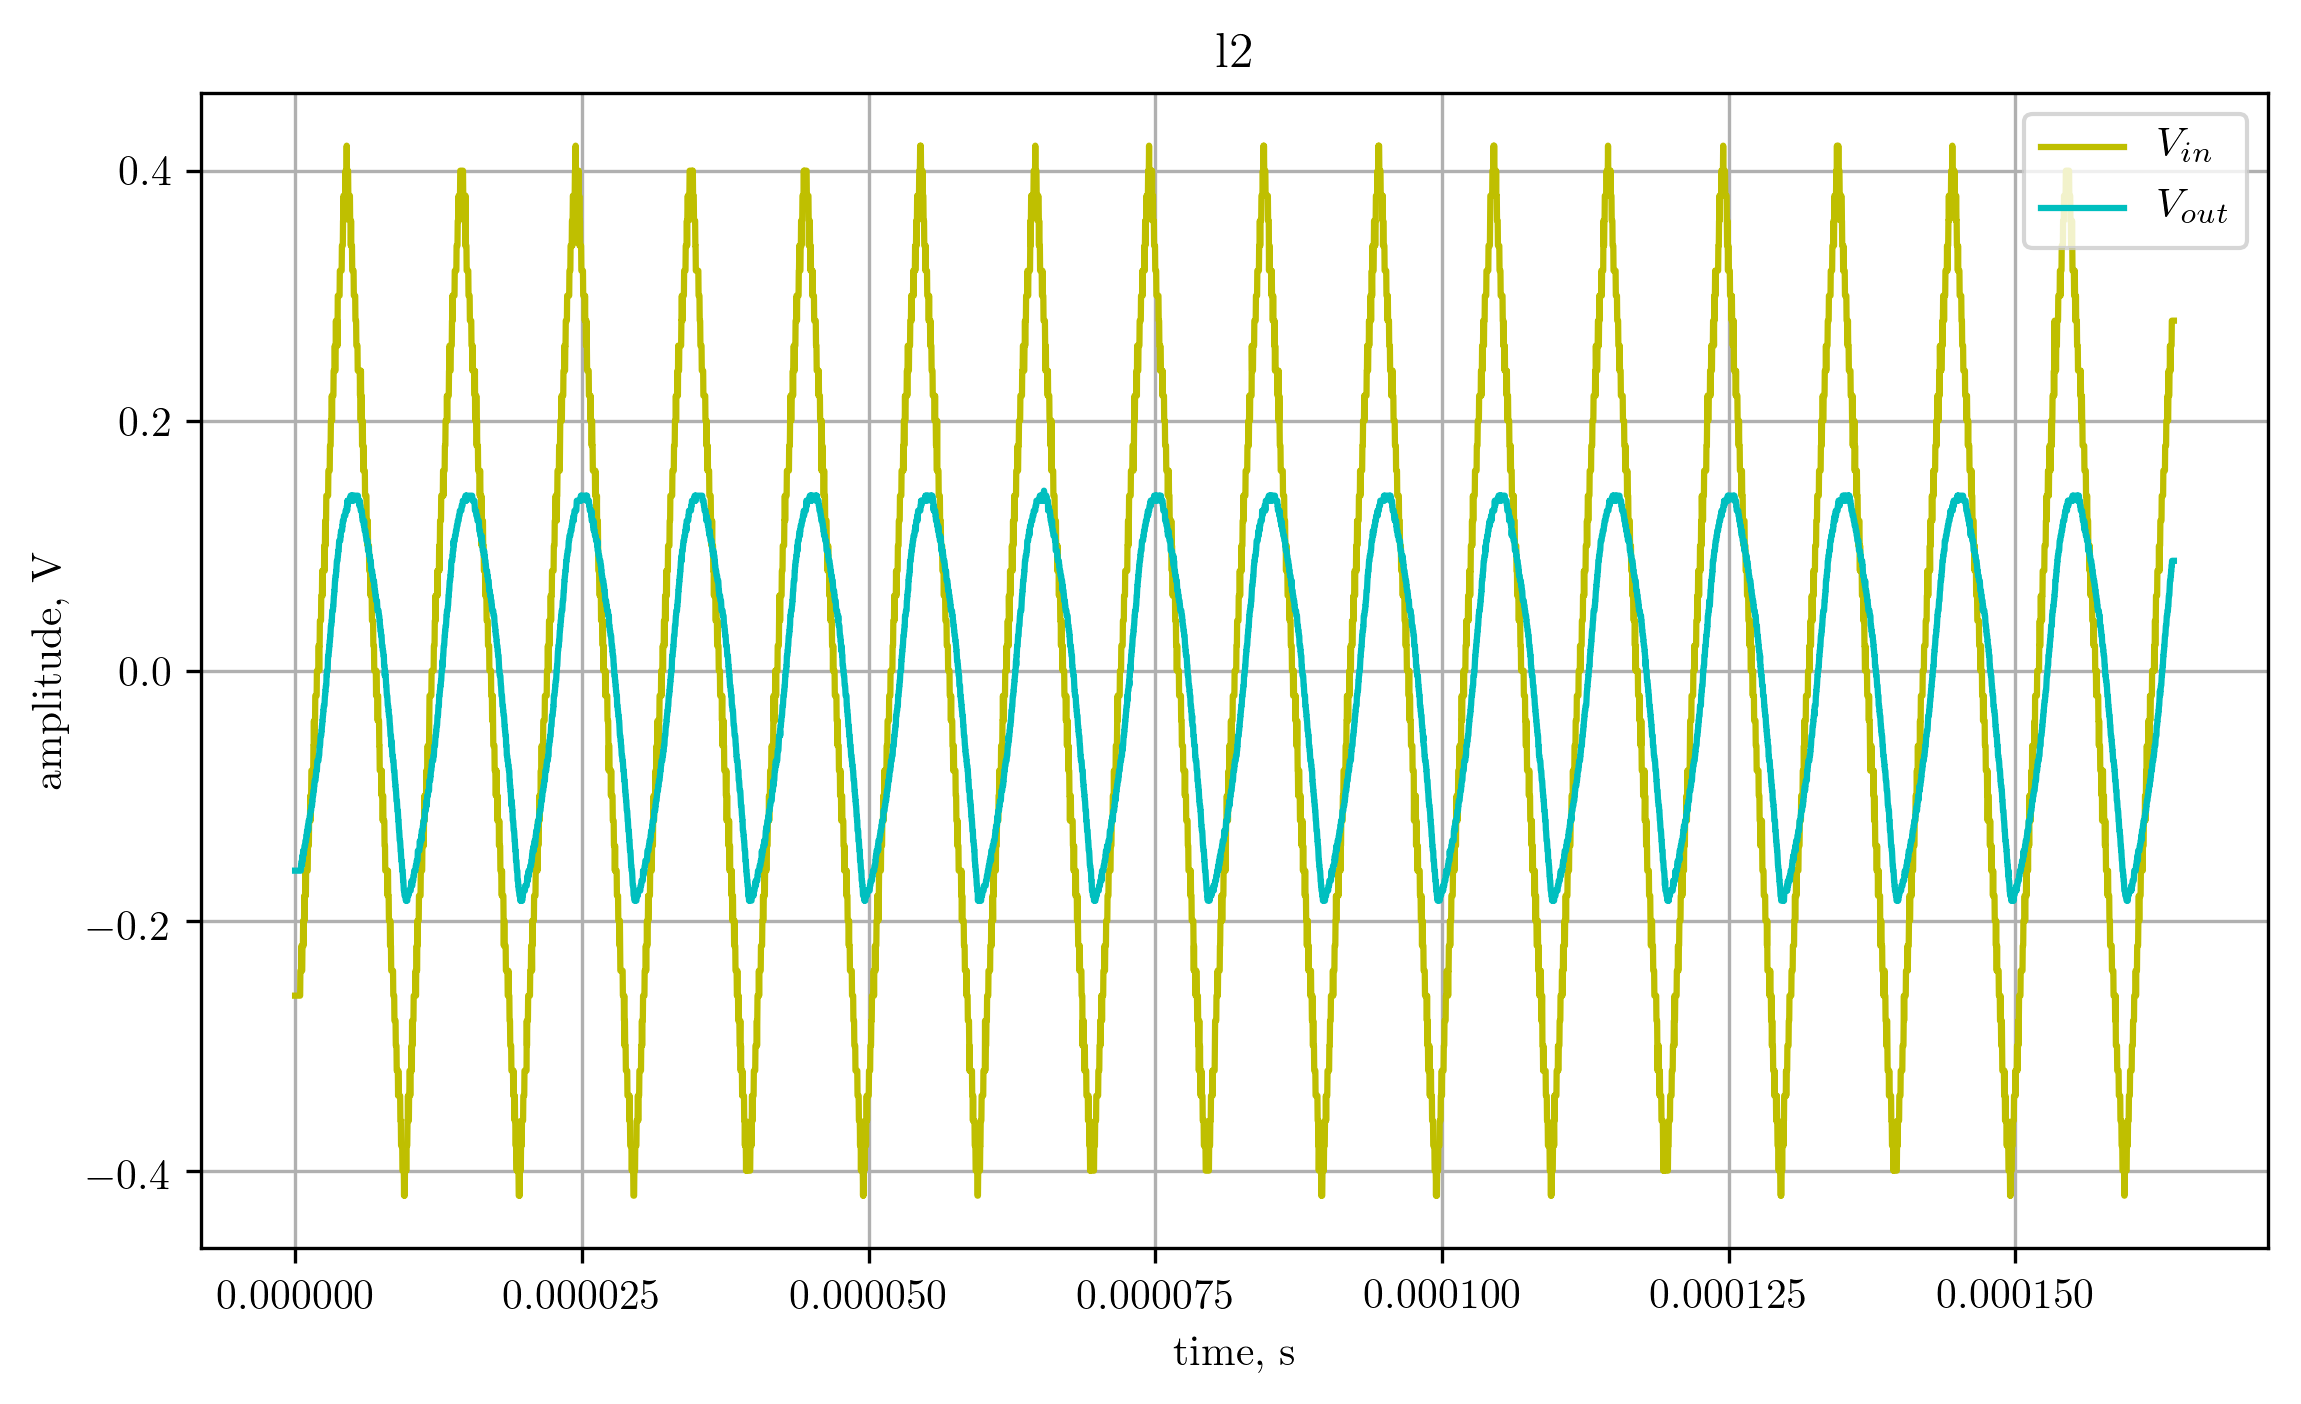
\includegraphics[width = \textwidth]{l2.png}
    \caption{Input-output curves of a Wheatstone bridge, $R_T$ replaced with an inductor, $V_{in} = 3.75$ V.}
    \label{fig:ind-hi}
\end{figure}

\end{document}